% Options for packages loaded elsewhere
\PassOptionsToPackage{unicode}{hyperref}
\PassOptionsToPackage{hyphens}{url}
%
\documentclass[
  a4paper,
]{article}
\usepackage{lmodern}
\usepackage{amssymb,amsmath}
\usepackage{ifxetex,ifluatex}
\ifnum 0\ifxetex 1\fi\ifluatex 1\fi=0 % if pdftex
  \usepackage[T1]{fontenc}
  \usepackage[utf8]{inputenc}
  \usepackage{textcomp} % provide euro and other symbols
\else % if luatex or xetex
  \usepackage{unicode-math}
  \defaultfontfeatures{Scale=MatchLowercase}
  \defaultfontfeatures[\rmfamily]{Ligatures=TeX,Scale=1}
\fi
% Use upquote if available, for straight quotes in verbatim environments
\IfFileExists{upquote.sty}{\usepackage{upquote}}{}
\IfFileExists{microtype.sty}{% use microtype if available
  \usepackage[]{microtype}
  \UseMicrotypeSet[protrusion]{basicmath} % disable protrusion for tt fonts
}{}
\makeatletter
\@ifundefined{KOMAClassName}{% if non-KOMA class
  \IfFileExists{parskip.sty}{%
    \usepackage{parskip}
  }{% else
    \setlength{\parindent}{0pt}
    \setlength{\parskip}{6pt plus 2pt minus 1pt}}
}{% if KOMA class
  \KOMAoptions{parskip=half}}
\makeatother
\usepackage{xcolor}
\IfFileExists{xurl.sty}{\usepackage{xurl}}{} % add URL line breaks if available
\IfFileExists{bookmark.sty}{\usepackage{bookmark}}{\usepackage{hyperref}}
\hypersetup{
  pdftitle={Lab 3},
  pdfauthor={Emilio Dorigatti},
  hidelinks,
  pdfcreator={LaTeX via pandoc}}
\urlstyle{same} % disable monospaced font for URLs
\usepackage[margin=1in]{geometry}
\usepackage{color}
\usepackage{fancyvrb}
\newcommand{\VerbBar}{|}
\newcommand{\VERB}{\Verb[commandchars=\\\{\}]}
\DefineVerbatimEnvironment{Highlighting}{Verbatim}{commandchars=\\\{\}}
% Add ',fontsize=\small' for more characters per line
\usepackage{framed}
\definecolor{shadecolor}{RGB}{248,248,248}
\newenvironment{Shaded}{\begin{snugshade}}{\end{snugshade}}
\newcommand{\AlertTok}[1]{\textcolor[rgb]{0.94,0.16,0.16}{#1}}
\newcommand{\AnnotationTok}[1]{\textcolor[rgb]{0.56,0.35,0.01}{\textbf{\textit{#1}}}}
\newcommand{\AttributeTok}[1]{\textcolor[rgb]{0.77,0.63,0.00}{#1}}
\newcommand{\BaseNTok}[1]{\textcolor[rgb]{0.00,0.00,0.81}{#1}}
\newcommand{\BuiltInTok}[1]{#1}
\newcommand{\CharTok}[1]{\textcolor[rgb]{0.31,0.60,0.02}{#1}}
\newcommand{\CommentTok}[1]{\textcolor[rgb]{0.56,0.35,0.01}{\textit{#1}}}
\newcommand{\CommentVarTok}[1]{\textcolor[rgb]{0.56,0.35,0.01}{\textbf{\textit{#1}}}}
\newcommand{\ConstantTok}[1]{\textcolor[rgb]{0.00,0.00,0.00}{#1}}
\newcommand{\ControlFlowTok}[1]{\textcolor[rgb]{0.13,0.29,0.53}{\textbf{#1}}}
\newcommand{\DataTypeTok}[1]{\textcolor[rgb]{0.13,0.29,0.53}{#1}}
\newcommand{\DecValTok}[1]{\textcolor[rgb]{0.00,0.00,0.81}{#1}}
\newcommand{\DocumentationTok}[1]{\textcolor[rgb]{0.56,0.35,0.01}{\textbf{\textit{#1}}}}
\newcommand{\ErrorTok}[1]{\textcolor[rgb]{0.64,0.00,0.00}{\textbf{#1}}}
\newcommand{\ExtensionTok}[1]{#1}
\newcommand{\FloatTok}[1]{\textcolor[rgb]{0.00,0.00,0.81}{#1}}
\newcommand{\FunctionTok}[1]{\textcolor[rgb]{0.00,0.00,0.00}{#1}}
\newcommand{\ImportTok}[1]{#1}
\newcommand{\InformationTok}[1]{\textcolor[rgb]{0.56,0.35,0.01}{\textbf{\textit{#1}}}}
\newcommand{\KeywordTok}[1]{\textcolor[rgb]{0.13,0.29,0.53}{\textbf{#1}}}
\newcommand{\NormalTok}[1]{#1}
\newcommand{\OperatorTok}[1]{\textcolor[rgb]{0.81,0.36,0.00}{\textbf{#1}}}
\newcommand{\OtherTok}[1]{\textcolor[rgb]{0.56,0.35,0.01}{#1}}
\newcommand{\PreprocessorTok}[1]{\textcolor[rgb]{0.56,0.35,0.01}{\textit{#1}}}
\newcommand{\RegionMarkerTok}[1]{#1}
\newcommand{\SpecialCharTok}[1]{\textcolor[rgb]{0.00,0.00,0.00}{#1}}
\newcommand{\SpecialStringTok}[1]{\textcolor[rgb]{0.31,0.60,0.02}{#1}}
\newcommand{\StringTok}[1]{\textcolor[rgb]{0.31,0.60,0.02}{#1}}
\newcommand{\VariableTok}[1]{\textcolor[rgb]{0.00,0.00,0.00}{#1}}
\newcommand{\VerbatimStringTok}[1]{\textcolor[rgb]{0.31,0.60,0.02}{#1}}
\newcommand{\WarningTok}[1]{\textcolor[rgb]{0.56,0.35,0.01}{\textbf{\textit{#1}}}}
\usepackage{longtable,booktabs}
% Correct order of tables after \paragraph or \subparagraph
\usepackage{etoolbox}
\makeatletter
\patchcmd\longtable{\par}{\if@noskipsec\mbox{}\fi\par}{}{}
\makeatother
% Allow footnotes in longtable head/foot
\IfFileExists{footnotehyper.sty}{\usepackage{footnotehyper}}{\usepackage{footnote}}
\makesavenoteenv{longtable}
\usepackage{graphicx}
\makeatletter
\def\maxwidth{\ifdim\Gin@nat@width>\linewidth\linewidth\else\Gin@nat@width\fi}
\def\maxheight{\ifdim\Gin@nat@height>\textheight\textheight\else\Gin@nat@height\fi}
\makeatother
% Scale images if necessary, so that they will not overflow the page
% margins by default, and it is still possible to overwrite the defaults
% using explicit options in \includegraphics[width, height, ...]{}
\setkeys{Gin}{width=\maxwidth,height=\maxheight,keepaspectratio}
% Set default figure placement to htbp
\makeatletter
\def\fps@figure{htbp}
\makeatother
\setlength{\emergencystretch}{3em} % prevent overfull lines
\providecommand{\tightlist}{%
  \setlength{\itemsep}{0pt}\setlength{\parskip}{0pt}}
\setcounter{secnumdepth}{-\maxdimen} % remove section numbering
\usepackage{bbold}
\usepackage{tikz}
\ifluatex
  \usepackage{selnolig}  % disable illegal ligatures
\fi

\title{Lab 3}
\author{Emilio Dorigatti}
\date{2020-11-20}

\begin{document}
\maketitle

Welcome to the third lab. The first exercise is an implementation of
gradient descent on a bivariate function. The second exercise is about
computing derivatives of the weights of a neural network, and the third
exercise combines the previous two.

\hypertarget{exercise-1}{%
\subsection{Exercise 1}\label{exercise-1}}

This exercise is about gradient descent. We will use the function
\(f(x_1, x_2)=(x_1-6)^2+x_2^2-x_1x_2\) as a running example:

\begin{enumerate}
\def\labelenumi{\arabic{enumi}.}
\tightlist
\item
  Use pen and paper to do three iterations of gradient descent:

  \begin{itemize}
  \tightlist
  \item
    Find the gradient of \(f\);
  \item
    Start from the point \(x_1=x_2=6\) and use a step size of \(1/2\)
    for the first step, \(1/3\) for the second step and \(1/4\) for the
    third step;
  \item
    What will happen if you keep going?
  \end{itemize}
\item
  Write a function that performs gradient descent:

  \begin{itemize}
  \tightlist
  \item
    For simplicity, we use a constant learning rate.
  \item
    Can you find a way to prematurely stop the optimization when you are
    close to the optimum?
  \end{itemize}
\end{enumerate}

\begin{Shaded}
\begin{Highlighting}[]
\NormalTok{func.value }\OtherTok{=} \ControlFlowTok{function}\NormalTok{(x) \{}
\NormalTok{  (x[}\DecValTok{1}\NormalTok{] }\SpecialCharTok{{-}} \DecValTok{6}\NormalTok{)}\SpecialCharTok{\^{}}\DecValTok{2}\SpecialCharTok{+}\NormalTok{x[}\DecValTok{2}\NormalTok{]}\SpecialCharTok{\^{}}\DecValTok{2}\SpecialCharTok{{-}}\NormalTok{x[}\DecValTok{1}\NormalTok{]}\SpecialCharTok{*}\NormalTok{x[}\DecValTok{2}\NormalTok{]}
\NormalTok{\}}

\NormalTok{func.gradient }\OtherTok{=} \ControlFlowTok{function}\NormalTok{(x) \{}
  \FunctionTok{c}\NormalTok{(}
    \DecValTok{2}\SpecialCharTok{*}\NormalTok{x[}\DecValTok{1}\NormalTok{]}\SpecialCharTok{{-}}\NormalTok{x[}\DecValTok{2}\NormalTok{]}\SpecialCharTok{{-}}\DecValTok{12}\NormalTok{,}
    \SpecialCharTok{{-}}\NormalTok{x[}\DecValTok{1}\NormalTok{]}\SpecialCharTok{+}\DecValTok{2}\SpecialCharTok{*}\NormalTok{x[}\DecValTok{2}\NormalTok{]}
\NormalTok{  )}
\NormalTok{\}}

\FunctionTok{func.value}\NormalTok{(}\FunctionTok{c}\NormalTok{(}\DecValTok{6}\NormalTok{, }\DecValTok{6}\NormalTok{))}
\end{Highlighting}
\end{Shaded}

\begin{verbatim}
## [1] 0
\end{verbatim}

\begin{Shaded}
\begin{Highlighting}[]
\FunctionTok{func.gradient}\NormalTok{(}\FunctionTok{c}\NormalTok{(}\DecValTok{6}\NormalTok{, }\DecValTok{6}\NormalTok{))}
\end{Highlighting}
\end{Shaded}

\begin{verbatim}
## [1] -6  6
\end{verbatim}

Does it match what you computed?

\begin{Shaded}
\begin{Highlighting}[]
\NormalTok{gradient\_descent\_optimizer }\OtherTok{=} \ControlFlowTok{function}\NormalTok{(x0, func, grad, max\_steps, alpha) \{}
  \CommentTok{\# x0 is the initial point}
  \CommentTok{\# func computes the value of the function at a given point}
  \CommentTok{\# grad computes the gradient of the function at a given point}
  \CommentTok{\# max\_steps is the maximum number of gradient descent steps}
  \CommentTok{\# alpha is the learning rate}
  
\NormalTok{  x }\OtherTok{=}\NormalTok{ x0}
\NormalTok{  v }\OtherTok{=} \FunctionTok{func}\NormalTok{(x0)}
  \ControlFlowTok{for}\NormalTok{(i }\ControlFlowTok{in} \DecValTok{1}\SpecialCharTok{:}\NormalTok{max\_steps) \{}
\NormalTok{    x }\OtherTok{=}\NormalTok{ x }\SpecialCharTok{{-}}\NormalTok{ alpha }\SpecialCharTok{*} \FunctionTok{grad}\NormalTok{(x)}
\NormalTok{    vnew }\OtherTok{=} \FunctionTok{func}\NormalTok{(x)}
    \ControlFlowTok{if}\NormalTok{(v }\SpecialCharTok{{-}}\NormalTok{ vnew }\SpecialCharTok{\textless{}} \FloatTok{1e{-}4}\NormalTok{) \{}
      \ControlFlowTok{break}
\NormalTok{    \}}
\NormalTok{    v }\OtherTok{=}\NormalTok{ vnew}
\NormalTok{  \}}
\NormalTok{  x}
\NormalTok{\}}

\FunctionTok{gradient\_descent\_optimizer}\NormalTok{(}\FunctionTok{c}\NormalTok{(}\DecValTok{6}\NormalTok{, }\DecValTok{6}\NormalTok{), func.value, func.gradient, }\DecValTok{10}\NormalTok{, }\FloatTok{0.1}\NormalTok{)}
\end{Highlighting}
\end{Shaded}

\begin{verbatim}
## [1] 7.943505 4.056495
\end{verbatim}

Play a bit with the starting point and learning rate to get a feel for
its behavior; how close can you get to the minimum?

\hypertarget{solution}{%
\subsubsection{Solution}\label{solution}}

The gradient of \(f\) is:

\[
\nabla_{\textbf{x}}f(\textbf{x})=\left\vert\begin{matrix}
\partial f/\partial x_1 \\
\partial f/\partial x_2 \\
\end{matrix}\right\vert=\left\vert\begin{matrix}
2(x_1-6)-x_2 \\
2x_2-x_1 \\
\end{matrix}\right\vert
\]

For \(\textbf{x}=|6,6|^T\) we have \(f(\textbf{x})=0\) and
\(\nabla_{\textbf{x}}f(\textbf{x})=|-6,6|^T\).

Let \(\textbf{x}^{(t)}\) denote the point at the \(t\)-th iteration.
Then:

\begin{longtable}[]{@{}lllll@{}}
\toprule
\begin{minipage}[b]{0.17\columnwidth}\raggedright
\(t\)\strut
\end{minipage} & \begin{minipage}[b]{0.17\columnwidth}\raggedright
\(\textbf{x}^{(t)}\)\strut
\end{minipage} & \begin{minipage}[b]{0.17\columnwidth}\raggedright
\(f(\textbf{x}^{(t)})\)\strut
\end{minipage} & \begin{minipage}[b]{0.17\columnwidth}\raggedright
\(\nabla_{\textbf{x}}f(\textbf{x})\)\strut
\end{minipage} & \begin{minipage}[b]{0.17\columnwidth}\raggedright
\(\textbf{x}^{(t+1)}\)\strut
\end{minipage}\tabularnewline
\midrule
\endhead
\begin{minipage}[t]{0.17\columnwidth}\raggedright
1\strut
\end{minipage} & \begin{minipage}[t]{0.17\columnwidth}\raggedright
\(|6,6|\)\strut
\end{minipage} & \begin{minipage}[t]{0.17\columnwidth}\raggedright
\(0\)\strut
\end{minipage} & \begin{minipage}[t]{0.17\columnwidth}\raggedright
\(|-6,6|\)\strut
\end{minipage} & \begin{minipage}[t]{0.17\columnwidth}\raggedright
\(|6,6|-(1/2)\cdot|-6,6|=|9,3|\)\strut
\end{minipage}\tabularnewline
\begin{minipage}[t]{0.17\columnwidth}\raggedright
2\strut
\end{minipage} & \begin{minipage}[t]{0.17\columnwidth}\raggedright
\(|9,3|\)\strut
\end{minipage} & \begin{minipage}[t]{0.17\columnwidth}\raggedright
\(-9\)\strut
\end{minipage} & \begin{minipage}[t]{0.17\columnwidth}\raggedright
\(|3,-3|\)\strut
\end{minipage} & \begin{minipage}[t]{0.17\columnwidth}\raggedright
\(|9,3|-(1/3)\cdot|3,-3|=|8,4|\)\strut
\end{minipage}\tabularnewline
\begin{minipage}[t]{0.17\columnwidth}\raggedright
3\strut
\end{minipage} & \begin{minipage}[t]{0.17\columnwidth}\raggedright
\(|8,4|\)\strut
\end{minipage} & \begin{minipage}[t]{0.17\columnwidth}\raggedright
\(-12\)\strut
\end{minipage} & \begin{minipage}[t]{0.17\columnwidth}\raggedright
\(|0,0|\)\strut
\end{minipage} & \begin{minipage}[t]{0.17\columnwidth}\raggedright
\(|8,4|-(1/4)\cdot|0,0|=|8,4|\)\strut
\end{minipage}\tabularnewline
\bottomrule
\end{longtable}

Where all vectors are intended to be vertical. As the gradient at the
last point is zero, nothing will change if we continue to apply this
procedure.

\hypertarget{exercise-2}{%
\subsection{Exercise 2}\label{exercise-2}}

This exercise is about computing gradients with the chain rule, with pen
and paper. We will work with a neural network with a single hidden layer
with two neurons and an output layer with one neuron (see Figure
\ref{fig:ex2net}).

\begin{figure}
\centering
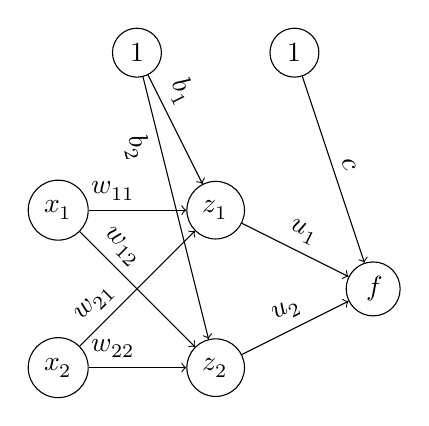
\begin{tikzpicture}
\node[draw, circle] (b1) at (1, 4) {$1$ };
\node[draw, circle] (x1) at (0, 2) {$x_1$ };
\node[draw, circle] (x2) at (0, 0) { $x_2$ };
\node[draw, circle] (b2) at (3, 4) { $1$ };
\node[draw, circle] (z1) at (2, 2) { $z_1$ };
\node[draw, circle] (z2) at (2, 0) { $z_2$ };
\node[draw, circle] (y) at (4, 1) { $f$ };

\draw[->] (b1) -- (z1) node [near start,above,sloped] { $b_1$ };
\draw[->] (b1) -- (z2) node [near start,below,sloped] { $b_2$ };

\draw[->] (x1) -- (z1) node [near start,above,sloped] { $w_{11}$ };
\draw[->] (x1) -- (z2) node [near start,above,sloped] { $w_{12}$ };

\draw[->] (x2) -- (z1) node [near start,above,sloped] { $w_{21}$ };
\draw[->] (x2) -- (z2) node [near start,above,sloped] { $w_{22}$ };

\draw[->] (b2) -- (y) node [midway,above,sloped] { $c$ };
\draw[->] (z1) -- (y) node [midway,above,sloped] { $u_1$ };
\draw[->] (z2) -- (y) node [midway,above,sloped] { $u_2$ };
\end{tikzpicture}
\caption{Neural network used in Exercise 2.}
\label{fig:ex2net}
\end{figure}

The neurons in the hidden layer use the \(\tanh\) activation, while the
output neuron uses the sigmoid. The loss used in binary classification
is the \emph{binary cross-entropy}:

\[
\mathcal{L}(y, f_{out})=-y\log f_{out}-(1-y)\log(1-f_{out})
\]

where \(y\in\{0,1\}\) is the true label and \(f_{out}\in(0,1)\) is the
predicted probability that \(y=1\).

\begin{enumerate}
\def\labelenumi{\arabic{enumi}.}
\tightlist
\item
  Compute \(\partial\mathcal{L}(y, f_{out})/\partial f_{out}\)
\item
  Compute \(\partial f_{out}/\partial f_{in}\)
\item
  Show that \(\partial\sigma(x)/\partial x=\sigma(x)(1-\sigma(x))\)
\item
  Show that \(\partial\tanh(x)/\partial x=1-\tanh(x)^2\) (Hint:
  \(\tanh(x)=(e^x-e^{-x})(e^x+e^{-x})^{-1}\))
\item
  Compute \(\partial f_{in}/\partial c\)
\item
  Compute \(\partial f_{in}/\partial u_1\)
\item
  Compute \(\partial\mathcal{L}(y, f_{out})/\partial c\)
\item
  Compute \(\partial\mathcal{L}(y, f_{out})/\partial u_1\)
\item
  Compute \(\partial f_{in}/\partial z_{2,out}\)
\item
  Compute \(\partial z_{2,out}/\partial z_{2,in}\)
\item
  Compute \(\partial z_{2,in}/\partial b_2\)
\item
  Compute \(\partial z_{2,in}/\partial w_{12}\)
\item
  Compute \(\partial z_{2,in}/\partial x_1\)
\item
  Compute \(\partial\mathcal{L}(y, f_{out})/\partial b_2\)
\item
  Compute \(\partial\mathcal{L}(y, f_{out})/\partial w_{12}\)
\item
  Compute \(\partial\mathcal{L}(y, f_{out})/\partial x_1\)
\end{enumerate}

You will notice that there are lots of redundancies. We will see how to
improve these computations in the lecture and in the next lab. Luckily,
modern deep learning software computes gradients automatically for you.

\hypertarget{solution-1}{%
\subsubsection{Solution}\label{solution-1}}

\hypertarget{question-1}{%
\paragraph{Question 1}\label{question-1}}

\begin{align*}
\frac{\partial\mathcal{L}(y,  f_{out})}{\partial f_{out}}
&=\frac{\partial}{\partial f_{out}}\bigg(y\log f_{out}+(1-y)\log(1- f_{out})\bigg)\\
&=-\frac{y}{ f_{out}}+\frac{1-y}{1- f_{out}}
\end{align*}

\hypertarget{question-2}{%
\paragraph{Question 2}\label{question-2}}

\begin{align*}
\frac{\partial f_{out}}{\partial f_{in}}
&=\frac{\partial}{\partial f_{in}} \frac{1}{1+e^{- f_{in}}} \\
&=-(1+e^{- f_{in}})^{-2}\cdot -e^{- f_{in}} \\
&=\frac{e^{- f_{in}}}{(1+e^{- f_{in}})^{2}}
\end{align*}

\hypertarget{question-3}{%
\paragraph{Question 3}\label{question-3}}

\begin{align*}
\frac{\partial}{\partial x} \frac{1}{1+e^{-x}}
&=\frac{e^{-x}}{(1+e^{-x})^2} \\
&=\frac{1}{1+e^{-x}} \cdot \frac{(1+e^{-x})-1}{1+e^{-x}} \\
&=\frac{1}{1+e^{-x}} \cdot \left(1-\frac{1}{1+e^{-x}}\right) \\
&=\sigma(x)(1-\sigma(x))
\end{align*}

\hypertarget{question-4}{%
\paragraph{Question 4}\label{question-4}}

\begin{align*}
\frac{\partial}{\partial x}\tanh(x)
&=\frac{\partial}{\partial x}\frac{e^x-e^{-x}}{e^x+e^{-x}} \\
&=\frac{(e^x+e^{-x})(e^x+e^{-x})-(e^x-e^{-x})(e^x-e^{-x})}{(e^x+e^{-x})^2} \\
&=1-\frac{(e^x-e^{-x})^2}{(e^x+e^{-x})^2} \\
\end{align*}

\hypertarget{question-5}{%
\paragraph{Question 5}\label{question-5}}

\begin{align*}
\frac{\partial f_{in}}{c}
&=\frac{\partial}{c}\left(c+u_1\cdot z_{1,out}+u_2\cdot z_{2,out}\right) \\
&=1
\end{align*}

\hypertarget{question-6}{%
\paragraph{Question 6}\label{question-6}}

\begin{align*}
\frac{\partial f_{in}}{u_1}
&=\frac{\partial}{u_1}\left(c+u_1\cdot z_{1,out}+u_2\cdot z_{2,out}\right) \\
&=z_{1,out}
\end{align*}

\hypertarget{question-7}{%
\paragraph{Question 7}\label{question-7}}

\begin{align*}
\frac{\partial\mathcal{L}(y,  f_{out})}{\partial c}
&=\frac{\partial\mathcal{L}(y,  f_{out})}{\partial f_{out}}
\cdot\frac{\partial f_{out}}{\partial f_{in}}
\cdot\frac{\partial f_{in}}{c} \\
&=\left(-\frac{y}{ f_{out}}+\frac{1-y}{1- f_{out}}\right)
\cdot\sigma(f_{in})(1-\sigma(f_{in}))
\cdot 1
\end{align*}

\hypertarget{question-8}{%
\paragraph{Question 8}\label{question-8}}

\begin{align*}
\frac{\partial\mathcal{L}(y,  f_{out})}{\partial u_1}
&=\frac{\partial\mathcal{L}(y,  f_{out})}{\partial f_{out}}
\cdot\frac{\partial f_{out}}{\partial f_{in}}
\cdot\frac{\partial f_{in}}{u_1} \\
&=\left(-\frac{y}{ f_{out}}+\frac{1-y}{1- f_{out}}\right)
\cdot\sigma(f_{in})(1-\sigma(f_{in}))
\cdot z_{1,out}
\end{align*}

\hypertarget{question-9}{%
\paragraph{Question 9}\label{question-9}}

\begin{align*}
\frac{\partial f_{in}}{\partial z_{2,out}}
&=\frac{\partial}{\partial z_{2,out}}\left(c+u_1\cdot z_{1,out}+u_2\cdot z_{2,out}\right) \\
&=u_2
\end{align*}

\hypertarget{question-10}{%
\paragraph{Question 10}\label{question-10}}

\begin{align*}
\frac{\partial z_{2,out}}{\partial z_{2,in}}
&=\frac{\partial}{\partial z_{2,in}}\sigma(z_{2,in})\\
&=1-\tanh(z_{2,in})^2
\end{align*}

\hypertarget{question-11}{%
\paragraph{Question 11}\label{question-11}}

\begin{align*}
\frac{\partial z_{2,in}}{\partial b_2}
&=\frac{\partial}{\partial b_2}\left(b_2+w_{12}\cdot x_1+w_{22}\cdot x_2 \right) \\
&=1
\end{align*}

\hypertarget{question-12}{%
\paragraph{Question 12}\label{question-12}}

\begin{align*}
\frac{\partial z_{2,in}}{\partial w_{12}}
&=\frac{\partial}{\partial b_2}\left(b_2+w_{12}\cdot x_1+w_{22}\cdot x_2 \right) \\
&=x_1
\end{align*}

\hypertarget{question-13}{%
\paragraph{Question 13}\label{question-13}}

\begin{align*}
\frac{\partial z_{2,in}}{\partial x_1}
&=\frac{\partial}{\partial x_1}\left(b_2+w_{12}\cdot x_1+w_{22}\cdot x_2 \right) \\
&=w_{12}
\end{align*}

\hypertarget{question-14}{%
\paragraph{Question 14}\label{question-14}}

\begin{align*}
\frac{\partial\mathcal{L}(y,  f_{out})}{\partial b_2}
&=\frac{\partial\mathcal{L}(y,  f_{out})}{\partial f_{out}}
\cdot\frac{\partial f_{out}}{\partial f_{in}}
\cdot\frac{\partial f_{in}}{\partial z_{2,out}}
\cdot\frac{\partial z_{2,out}}{\partial z_{2,in}}
\cdot\frac{\partial z_{2,in}}{\partial b_2} \\
&=\left(-\frac{y}{ f_{out}}+\frac{1-y}{1- f_{out}}\right)
\cdot\sigma(f_{in})(1-\sigma(f_{in}))
\cdot u_2
\cdot(1-\tanh(z_{2,in})^2)
\cdot 1
\end{align*}

\hypertarget{question-15}{%
\paragraph{Question 15}\label{question-15}}

\begin{align*}
\frac{\partial\mathcal{L}(y,  f_{out})}{\partial w_{12}}
&=\frac{\partial\mathcal{L}(y,  f_{out})}{\partial f_{out}}
\cdot\frac{\partial f_{out}}{\partial f_{in}}
\cdot\frac{\partial f_{in}}{\partial z_{2,out}}
\cdot\frac{\partial z_{2,out}}{\partial z_{2,in}}
\cdot\frac{\partial z_{2,in}}{\partial w_{12}} \\
&=\left(-\frac{y}{ f_{out}}+\frac{1-y}{1- f_{out}}\right)
\cdot\sigma(f_{in})(1-\sigma(f_{in}))
\cdot u_2
\cdot(1-\tanh(z_{2,in})^2)
\cdot x_1
\end{align*}

\hypertarget{question-16}{%
\paragraph{Question 16}\label{question-16}}

\begin{align*}
\frac{\partial\mathcal{L}(y,  f_{out})}{\partial x_1}
&=\frac{\partial\mathcal{L}(y,  f_{out})}{\partial f_{out}}
\cdot\frac{\partial f_{out}}{\partial f_{in}}
\cdot\frac{\partial f_{in}}{\partial z_{2,out}}
\cdot\frac{\partial z_{2,out}}{\partial z_{2,in}}
\cdot\frac{\partial z_{2,in}}{\partial x_{1}} \\
&\quad\quad + \frac{\partial\mathcal{L}(y,  f_{out})}{\partial f_{out}}
\cdot\frac{\partial f_{out}}{\partial f_{in}}
\cdot\frac{\partial f_{in}}{\partial z_{1,out}}
\cdot\frac{\partial z_{1,out}}{\partial z_{1,in}}
\cdot\frac{\partial z_{1,in}}{\partial x_{1}} \\
&=\left(-\frac{y}{ f_{out}}+\frac{1-y}{1- f_{out}}\right)
\cdot\sigma(f_{in})(1-\sigma(f_{in}))
\cdot u_2
\cdot(1-\tanh(z_{2,in})^2)
\cdot w_{12} \\
&\quad\quad+\left(-\frac{y}{ f_{out}}+\frac{1-y}{1- f_{out}}\right)
\cdot\sigma(f_{in})(1-\sigma(f_{in}))
\cdot u_1
\cdot(1-\tanh(z_{1,in})^2)
\cdot w_{11}
\end{align*}

\hypertarget{exercise-3}{%
\subsection{Exercise 3}\label{exercise-3}}

Now that we know how to do gradient descent and how to compute the
derivatives of the weights of a simple network, we can try to do these
steps together and train our first neural network! We will use the small
dataset with five points we studied in the first lab.

First, let's define the dataset:

\begin{Shaded}
\begin{Highlighting}[]
\NormalTok{data.x1 }\OtherTok{=} \FunctionTok{c}\NormalTok{(}\DecValTok{0}\NormalTok{, }\DecValTok{1}\NormalTok{, }\DecValTok{0}\NormalTok{, }\SpecialCharTok{{-}}\DecValTok{1}\NormalTok{, }\DecValTok{0}\NormalTok{);}
\NormalTok{data.x2 }\OtherTok{=} \FunctionTok{c}\NormalTok{(}\DecValTok{0}\NormalTok{, }\DecValTok{0}\NormalTok{, }\SpecialCharTok{{-}}\DecValTok{1}\NormalTok{, }\DecValTok{0}\NormalTok{, }\DecValTok{1}\NormalTok{);}
\NormalTok{data.y }\OtherTok{=} \FunctionTok{c}\NormalTok{(}\DecValTok{1}\NormalTok{, }\DecValTok{0}\NormalTok{, }\DecValTok{0}\NormalTok{, }\DecValTok{0}\NormalTok{, }\DecValTok{0}\NormalTok{);}
\end{Highlighting}
\end{Shaded}

Next, a function to compute the output of the network:

\begin{Shaded}
\begin{Highlighting}[]
\NormalTok{sigmoid }\OtherTok{=} \ControlFlowTok{function}\NormalTok{(x) \{}
  \DecValTok{1} \SpecialCharTok{/}\NormalTok{ (}\DecValTok{1} \SpecialCharTok{+} \FunctionTok{exp}\NormalTok{(}\SpecialCharTok{{-}}\NormalTok{x))}
\NormalTok{\}}

\NormalTok{nnet.predict }\OtherTok{=} \ControlFlowTok{function}\NormalTok{(params) \{}
  \CommentTok{\# params is a vector, we first unpack for clarity}
\NormalTok{  b1 }\OtherTok{=}\NormalTok{ params[}\DecValTok{1}\NormalTok{]; b2 }\OtherTok{=}\NormalTok{ params[}\DecValTok{2}\NormalTok{];}
\NormalTok{  w11 }\OtherTok{=}\NormalTok{ params[}\DecValTok{3}\NormalTok{]; w12 }\OtherTok{=}\NormalTok{ params[}\DecValTok{4}\NormalTok{];}
\NormalTok{  w21 }\OtherTok{=}\NormalTok{ params[}\DecValTok{5}\NormalTok{]; w22 }\OtherTok{=}\NormalTok{ params[}\DecValTok{6}\NormalTok{];}
\NormalTok{  c }\OtherTok{=}\NormalTok{ params[}\DecValTok{7}\NormalTok{]; u1 }\OtherTok{=}\NormalTok{ params[}\DecValTok{8}\NormalTok{]; u2 }\OtherTok{=}\NormalTok{ params[}\DecValTok{9}\NormalTok{];}
  
\NormalTok{  z1 }\OtherTok{=} \FunctionTok{tanh}\NormalTok{(b1 }\SpecialCharTok{+}\NormalTok{ data.x1 }\SpecialCharTok{*}\NormalTok{ w11 }\SpecialCharTok{+}\NormalTok{ data.x2 }\SpecialCharTok{*}\NormalTok{ w21)}
\NormalTok{  z2 }\OtherTok{=} \FunctionTok{tanh}\NormalTok{(b2 }\SpecialCharTok{+}\NormalTok{ data.x1 }\SpecialCharTok{*}\NormalTok{ w12 }\SpecialCharTok{+}\NormalTok{ data.x2 }\SpecialCharTok{*}\NormalTok{ w22)}
\NormalTok{  f }\OtherTok{=} \FunctionTok{sigmoid}\NormalTok{(c }\SpecialCharTok{+}\NormalTok{ u1 }\SpecialCharTok{*}\NormalTok{ z1 }\SpecialCharTok{+}\NormalTok{ u2 }\SpecialCharTok{*}\NormalTok{ z2)}
\NormalTok{  f}
\NormalTok{\}}

\CommentTok{\# this should return the predictions for the five points in the datasets}
\NormalTok{params }\OtherTok{=} \FunctionTok{rnorm}\NormalTok{(}\DecValTok{9}\NormalTok{)}
\FunctionTok{nnet.predict}\NormalTok{(params)}
\end{Highlighting}
\end{Shaded}

\begin{verbatim}
## [1] 0.4491225 0.4965392 0.5436179 0.3752571 0.4099662
\end{verbatim}

Since gradient descent is done on the loss function, we need a function
to compute it:

\begin{Shaded}
\begin{Highlighting}[]
\NormalTok{nnet.loss }\OtherTok{=} \ControlFlowTok{function}\NormalTok{(params) \{}
\NormalTok{  preds }\OtherTok{=} \FunctionTok{nnet.predict}\NormalTok{(params)}
  \SpecialCharTok{{-}}\FunctionTok{mean}\NormalTok{(data.y }\SpecialCharTok{*} \FunctionTok{log}\NormalTok{(preds }\SpecialCharTok{+} \FloatTok{1e{-}15}\NormalTok{) }\SpecialCharTok{+}\NormalTok{ (}\DecValTok{1} \SpecialCharTok{{-}}\NormalTok{ data.y) }\SpecialCharTok{*} \FunctionTok{log}\NormalTok{(}\DecValTok{1} \SpecialCharTok{{-}}\NormalTok{ preds }\SpecialCharTok{+} \FloatTok{1e{-}15}\NormalTok{))}
\NormalTok{\}}

\FunctionTok{nnet.loss}\NormalTok{(params)}
\end{Highlighting}
\end{Shaded}

\begin{verbatim}
## [1] 0.6538249
\end{verbatim}

Now, we need to compute the gradient of each parameter:

\begin{Shaded}
\begin{Highlighting}[]
\NormalTok{nnet.gradient }\OtherTok{=} \ControlFlowTok{function}\NormalTok{(params) \{}
  \CommentTok{\# params is a vector, we first unpack for clarity}
\NormalTok{  b1 }\OtherTok{=}\NormalTok{ params[}\DecValTok{1}\NormalTok{]; b2 }\OtherTok{=}\NormalTok{ params[}\DecValTok{2}\NormalTok{];}
\NormalTok{  w11 }\OtherTok{=}\NormalTok{ params[}\DecValTok{3}\NormalTok{]; w12 }\OtherTok{=}\NormalTok{ params[}\DecValTok{4}\NormalTok{];}
\NormalTok{  w21 }\OtherTok{=}\NormalTok{ params[}\DecValTok{5}\NormalTok{]; w22 }\OtherTok{=}\NormalTok{ params[}\DecValTok{6}\NormalTok{];}
\NormalTok{  c }\OtherTok{=}\NormalTok{ params[}\DecValTok{7}\NormalTok{]; u1 }\OtherTok{=}\NormalTok{ params[}\DecValTok{8}\NormalTok{]; u2 }\OtherTok{=}\NormalTok{ params[}\DecValTok{9}\NormalTok{];}
  
  \CommentTok{\# first, we perform the forward pass}
\NormalTok{  z1in }\OtherTok{=}\NormalTok{ b1 }\SpecialCharTok{+}\NormalTok{ data.x1 }\SpecialCharTok{*}\NormalTok{ w11 }\SpecialCharTok{+}\NormalTok{ data.x2 }\SpecialCharTok{*}\NormalTok{ w21}
\NormalTok{  z1out }\OtherTok{=} \FunctionTok{tanh}\NormalTok{(z1in)}
  
\NormalTok{  z2in }\OtherTok{=}\NormalTok{ b2 }\SpecialCharTok{+}\NormalTok{ data.x1 }\SpecialCharTok{*}\NormalTok{ w12 }\SpecialCharTok{+}\NormalTok{ data.x2 }\SpecialCharTok{*}\NormalTok{ w22}
\NormalTok{  z2out }\OtherTok{=} \FunctionTok{tanh}\NormalTok{(z2in)}
  
\NormalTok{  fin }\OtherTok{=}\NormalTok{ c }\SpecialCharTok{+}\NormalTok{ u1 }\SpecialCharTok{*}\NormalTok{ z1out }\SpecialCharTok{+}\NormalTok{ u2 }\SpecialCharTok{*}\NormalTok{ z2out}
\NormalTok{  fout }\OtherTok{=} \FunctionTok{sigmoid}\NormalTok{(fin)}
  
  \CommentTok{\# now we start back{-}propagation through the loss and the output neuron}
\NormalTok{  dL\_dfout }\OtherTok{=} \SpecialCharTok{{-}}\NormalTok{data.y }\SpecialCharTok{/}\NormalTok{ (fout }\SpecialCharTok{+} \FloatTok{1e{-}15}\NormalTok{) }\SpecialCharTok{+}\NormalTok{ (}\DecValTok{1} \SpecialCharTok{{-}}\NormalTok{ data.y) }\SpecialCharTok{/}\NormalTok{ (}\DecValTok{1} \SpecialCharTok{{-}}\NormalTok{ fout }\SpecialCharTok{+} \FloatTok{1e{-}15}\NormalTok{)}
\NormalTok{  dfout\_dfin }\OtherTok{=} \FunctionTok{sigmoid}\NormalTok{(fin) }\SpecialCharTok{*}\NormalTok{ (}\DecValTok{1} \SpecialCharTok{{-}} \FunctionTok{sigmoid}\NormalTok{(fin))}
  
  \CommentTok{\# compute the gradients for the parameters of the output layer}
\NormalTok{  dfin\_dc }\OtherTok{=} \DecValTok{1}
\NormalTok{  dfin\_du1 }\OtherTok{=}\NormalTok{ z1out}
\NormalTok{  dfin\_du2 }\OtherTok{=}\NormalTok{ z2out}
  \CommentTok{\# take the mean gradient across data points}
\NormalTok{  dL\_dc }\OtherTok{=} \FunctionTok{mean}\NormalTok{(dL\_dfout }\SpecialCharTok{*}\NormalTok{ dfout\_dfin }\SpecialCharTok{*}\NormalTok{ dfin\_dc)}
\NormalTok{  dL\_du1 }\OtherTok{=} \FunctionTok{mean}\NormalTok{(dL\_dfout }\SpecialCharTok{*}\NormalTok{ dfout\_dfin }\SpecialCharTok{*}\NormalTok{ dfin\_du1)}
\NormalTok{  dL\_du2 }\OtherTok{=} \FunctionTok{mean}\NormalTok{(dL\_dfout }\SpecialCharTok{*}\NormalTok{ dfout\_dfin }\SpecialCharTok{*}\NormalTok{ dfin\_du2)}
  
  \CommentTok{\# back{-}propagate through the neurons in the first hidden layer}
\NormalTok{  dfin\_dz1out }\OtherTok{=}\NormalTok{ u1}
\NormalTok{  dfin\_dz2out }\OtherTok{=}\NormalTok{ u2}
  
\NormalTok{  dz1out\_dz1in }\OtherTok{=} \DecValTok{1} \SpecialCharTok{{-}} \FunctionTok{tanh}\NormalTok{(z1in)}\SpecialCharTok{\^{}}\DecValTok{2}
\NormalTok{  dz2out\_dz2in }\OtherTok{=} \DecValTok{1} \SpecialCharTok{{-}} \FunctionTok{tanh}\NormalTok{(z2in)}\SpecialCharTok{\^{}}\DecValTok{2}
  
  \CommentTok{\# and compute the derivatives of the parameters of the hidden layer}
\NormalTok{  dz1in\_db1 }\OtherTok{=}\NormalTok{ dz2in\_db2 }\OtherTok{=} \DecValTok{1}
\NormalTok{  dL\_db1 }\OtherTok{=} \FunctionTok{mean}\NormalTok{(dL\_dfout }\SpecialCharTok{*}\NormalTok{ dfout\_dfin }\SpecialCharTok{*}\NormalTok{ dfin\_dz1out }\SpecialCharTok{*}\NormalTok{ dz1out\_dz1in }\SpecialCharTok{*}\NormalTok{ dz1in\_db1)}
\NormalTok{  dL\_db2 }\OtherTok{=} \FunctionTok{mean}\NormalTok{(dL\_dfout }\SpecialCharTok{*}\NormalTok{ dfout\_dfin }\SpecialCharTok{*}\NormalTok{ dfin\_dz2out }\SpecialCharTok{*}\NormalTok{ dz2out\_dz2in }\SpecialCharTok{*}\NormalTok{ dz2in\_db2)}
  
\NormalTok{  dz1in\_dw11 }\OtherTok{=}\NormalTok{ dz2in\_dw12 }\OtherTok{=}\NormalTok{ data.x1}
\NormalTok{  dL\_dw11 }\OtherTok{=} \FunctionTok{mean}\NormalTok{(dL\_dfout }\SpecialCharTok{*}\NormalTok{ dfout\_dfin }\SpecialCharTok{*}\NormalTok{ dfin\_dz1out }\SpecialCharTok{*}\NormalTok{ dz1out\_dz1in }\SpecialCharTok{*}\NormalTok{ dz1in\_dw11)}
\NormalTok{  dL\_dw12 }\OtherTok{=} \FunctionTok{mean}\NormalTok{(dL\_dfout }\SpecialCharTok{*}\NormalTok{ dfout\_dfin }\SpecialCharTok{*}\NormalTok{ dfin\_dz2out }\SpecialCharTok{*}\NormalTok{ dz2out\_dz2in }\SpecialCharTok{*}\NormalTok{ dz2in\_dw12)}
  
\NormalTok{  dz1in\_dw21 }\OtherTok{=}\NormalTok{ dz2in\_dw22 }\OtherTok{=}\NormalTok{ data.x2}
\NormalTok{  dL\_dw21 }\OtherTok{=} \FunctionTok{mean}\NormalTok{(dL\_dfout }\SpecialCharTok{*}\NormalTok{ dfout\_dfin }\SpecialCharTok{*}\NormalTok{ dfin\_dz1out }\SpecialCharTok{*}\NormalTok{ dz1out\_dz1in }\SpecialCharTok{*}\NormalTok{ dz1in\_dw21)}
\NormalTok{  dL\_dw22 }\OtherTok{=} \FunctionTok{mean}\NormalTok{(dL\_dfout }\SpecialCharTok{*}\NormalTok{ dfout\_dfin }\SpecialCharTok{*}\NormalTok{ dfin\_dz2out }\SpecialCharTok{*}\NormalTok{ dz2out\_dz2in }\SpecialCharTok{*}\NormalTok{ dz2in\_dw22)}
  
  \CommentTok{\# return the derivatives in the same order as the parameters vector}
  \FunctionTok{c}\NormalTok{(}
\NormalTok{    dL\_db1, dL\_db2,}
\NormalTok{    dL\_dw11, dL\_dw12,}
\NormalTok{    dL\_dw21, dL\_dw22,}
\NormalTok{    dL\_dc, dL\_du1, dL\_du2}
\NormalTok{  )}
\NormalTok{\}}

\FunctionTok{nnet.gradient}\NormalTok{(params)}
\end{Highlighting}
\end{Shaded}

\begin{verbatim}
## [1]  0.10535249 -0.16134603 -0.03237562  0.03281629 -0.06440284  0.05575347
## [7]  0.25490058 -0.04360869 -0.06480158
\end{verbatim}

Finite differences are a useful way to check that the gradients are
computed correctly:

\begin{Shaded}
\begin{Highlighting}[]
\CommentTok{\# first, compute the analytical gradient of the parameters}
\NormalTok{gradient }\OtherTok{=} \FunctionTok{nnet.gradient}\NormalTok{(params);}

\NormalTok{eps }\OtherTok{=} \FloatTok{1e{-}9}
\ControlFlowTok{for}\NormalTok{(i }\ControlFlowTok{in} \DecValTok{1}\SpecialCharTok{:}\DecValTok{9}\NormalTok{) \{}
  \CommentTok{\# compute loss when subtracting eps to parameter i}
\NormalTok{  neg\_params }\OtherTok{=} \FunctionTok{c}\NormalTok{(params);}
\NormalTok{  neg\_params[i] }\OtherTok{=}\NormalTok{ neg\_params[i] }\SpecialCharTok{{-}}\NormalTok{ eps;}
\NormalTok{  neg\_value }\OtherTok{=} \FunctionTok{nnet.loss}\NormalTok{(neg\_params);}
  
  \CommentTok{\# compute loss when adding eps to parameter i}
\NormalTok{  pos\_params }\OtherTok{=} \FunctionTok{c}\NormalTok{(params);}
\NormalTok{  pos\_params[i] }\OtherTok{=}\NormalTok{ pos\_params[i] }\SpecialCharTok{+}\NormalTok{ eps;}
\NormalTok{  pos\_value }\OtherTok{=} \FunctionTok{nnet.loss}\NormalTok{(pos\_params);}

  \CommentTok{\# compute the "empirical" gradient of parameter i}
\NormalTok{  fdiff\_gradient }\OtherTok{=} \FunctionTok{mean}\NormalTok{((pos\_value }\SpecialCharTok{{-}}\NormalTok{ neg\_value) }\SpecialCharTok{/}\NormalTok{ (}\DecValTok{2} \SpecialCharTok{*}\NormalTok{ eps));}
  
  \CommentTok{\# error if difference is too large}
  \FunctionTok{stopifnot}\NormalTok{(}\FunctionTok{abs}\NormalTok{(gradient[i] }\SpecialCharTok{{-}}\NormalTok{ fdiff\_gradient) }\SpecialCharTok{\textless{}} \FloatTok{1e{-}5}\NormalTok{);}
\NormalTok{\}}

\FunctionTok{print}\NormalTok{(}\StringTok{"Gradients are correct!"}\NormalTok{)}
\end{Highlighting}
\end{Shaded}

\begin{verbatim}
## [1] "Gradients are correct!"
\end{verbatim}

We can finally train our network. Since the network is so small compared
to the dataset, the training procedure is very sensitive to the way the
weights are initialized and the step size used in gradient descent.

Try to play around with the learning rate and the random initialization
of the weights and find reliable values that make training successful in
most cases.

\begin{Shaded}
\begin{Highlighting}[]
\NormalTok{min\_loss }\OtherTok{=} \DecValTok{10}
\NormalTok{best\_params }\OtherTok{=} \ConstantTok{NULL}

\ControlFlowTok{for}\NormalTok{(i }\ControlFlowTok{in} \DecValTok{1}\SpecialCharTok{:}\DecValTok{10}\NormalTok{) \{}
\NormalTok{  params }\OtherTok{=} \FunctionTok{rnorm}\NormalTok{(}\DecValTok{9}\NormalTok{, }\AttributeTok{sd =} \DecValTok{1}\NormalTok{)}
\NormalTok{  optimized\_params }\OtherTok{=} \FunctionTok{gradient\_descent\_optimizer}\NormalTok{(}
\NormalTok{    params, nnet.loss, nnet.gradient, }\AttributeTok{max\_steps =} \DecValTok{100}\NormalTok{, }\AttributeTok{alpha =} \DecValTok{1}
\NormalTok{  )}
\NormalTok{  final\_loss }\OtherTok{=} \FunctionTok{nnet.loss}\NormalTok{(optimized\_params)}
  \FunctionTok{cat}\NormalTok{(}\StringTok{"Loss"}\NormalTok{, final\_loss, }\FunctionTok{ifelse}\NormalTok{(final\_loss }\SpecialCharTok{\textless{}} \FloatTok{0.1}\NormalTok{, }\StringTok{"*"}\NormalTok{, }\StringTok{""}\NormalTok{), }\StringTok{"}\SpecialCharTok{\textbackslash{}n}\StringTok{"}\NormalTok{)}
  
  \ControlFlowTok{if}\NormalTok{(final\_loss }\SpecialCharTok{\textless{}}\NormalTok{ min\_loss) \{}
\NormalTok{    min\_loss }\OtherTok{=}\NormalTok{ final\_loss}
\NormalTok{    best\_params }\OtherTok{=}\NormalTok{ optimized\_params}
\NormalTok{  \}}
\NormalTok{\}}
\end{Highlighting}
\end{Shaded}

\begin{verbatim}
## Loss 0.4603099  
## Loss 0.09263696 * 
## Loss 0.162037  
## Loss 0.3783302  
## Loss 0.4366499  
## Loss 0.04427358 * 
## Loss 0.4067504  
## Loss 0.06471511 * 
## Loss 0.1449693  
## Loss 0.05334381 *
\end{verbatim}

We can use the function in the previous lab to visualize the decision
boundary of the best network:

\begin{Shaded}
\begin{Highlighting}[]
\FunctionTok{library}\NormalTok{(scales)}
\FunctionTok{library}\NormalTok{(ggplot2)}

\NormalTok{data }\OtherTok{=} \FunctionTok{as.matrix}\NormalTok{(}\FunctionTok{expand.grid}\NormalTok{(}
  \AttributeTok{x0 =} \DecValTok{1}\SpecialCharTok{:}\DecValTok{1}\NormalTok{,}
  \AttributeTok{x1 =} \FunctionTok{seq}\NormalTok{(}\SpecialCharTok{{-}}\DecValTok{2}\NormalTok{, }\DecValTok{2}\NormalTok{, }\DecValTok{1} \SpecialCharTok{/} \DecValTok{25}\NormalTok{),}
  \AttributeTok{x2 =} \FunctionTok{seq}\NormalTok{(}\SpecialCharTok{{-}}\DecValTok{2}\NormalTok{, }\DecValTok{2}\NormalTok{, }\DecValTok{1} \SpecialCharTok{/} \DecValTok{25}\NormalTok{)}
\NormalTok{))}

\NormalTok{data.x1 }\OtherTok{=}\NormalTok{ data[,}\DecValTok{2}\NormalTok{]}
\NormalTok{data.x2 }\OtherTok{=}\NormalTok{ data[,}\DecValTok{3}\NormalTok{]}

\NormalTok{plot\_grid }\OtherTok{=} \ControlFlowTok{function}\NormalTok{(predictions) \{}
  \CommentTok{\# plots the predicted value for each point on the grid;}
  \CommentTok{\# the predictions should have one column and}
  \CommentTok{\# the same number of rows (10,201) as the data}
\NormalTok{  df }\OtherTok{=} \FunctionTok{cbind}\NormalTok{(}\FunctionTok{as.data.frame}\NormalTok{(data), }\AttributeTok{y =}\NormalTok{ predictions)}
  \FunctionTok{ggplot}\NormalTok{() }\SpecialCharTok{+}
    \FunctionTok{geom\_tile}\NormalTok{(}\FunctionTok{aes}\NormalTok{(}\AttributeTok{x =}\NormalTok{ x1, }\AttributeTok{y =}\NormalTok{ x2, }\AttributeTok{fill =}\NormalTok{ y, }\AttributeTok{color =}\NormalTok{ y), df) }\SpecialCharTok{+}
    \FunctionTok{scale\_color\_gradient2}\NormalTok{(}\AttributeTok{low =} \FunctionTok{muted}\NormalTok{(}\StringTok{"blue"}\NormalTok{, }\DecValTok{70}\NormalTok{), }\AttributeTok{mid =} \StringTok{"white"}\NormalTok{,}
                         \AttributeTok{high =} \FunctionTok{muted}\NormalTok{(}\StringTok{"red"}\NormalTok{, }\DecValTok{70}\NormalTok{), }\AttributeTok{limits =} \FunctionTok{c}\NormalTok{(}\DecValTok{0}\NormalTok{, }\DecValTok{1}\NormalTok{),}
                         \AttributeTok{midpoint =} \FloatTok{0.5}\NormalTok{) }\SpecialCharTok{+}
    \FunctionTok{scale\_fill\_gradient2}\NormalTok{(}\AttributeTok{low =} \FunctionTok{muted}\NormalTok{(}\StringTok{"blue"}\NormalTok{, }\DecValTok{70}\NormalTok{), }\AttributeTok{mid =} \StringTok{"white"}\NormalTok{,}
                        \AttributeTok{high =} \FunctionTok{muted}\NormalTok{(}\StringTok{"red"}\NormalTok{, }\DecValTok{70}\NormalTok{), }\AttributeTok{limits =} \FunctionTok{c}\NormalTok{(}\DecValTok{0}\NormalTok{, }\DecValTok{1}\NormalTok{),}
                        \AttributeTok{midpoint =} \FloatTok{0.5}\NormalTok{) }\SpecialCharTok{+}
    \FunctionTok{geom\_point}\NormalTok{(}\FunctionTok{aes}\NormalTok{(}\AttributeTok{x=}\FunctionTok{c}\NormalTok{(}\DecValTok{0}\NormalTok{, }\DecValTok{1}\NormalTok{, }\DecValTok{0}\NormalTok{, }\SpecialCharTok{{-}}\DecValTok{1}\NormalTok{, }\DecValTok{0}\NormalTok{), }\AttributeTok{y=}\FunctionTok{c}\NormalTok{(}\DecValTok{0}\NormalTok{, }\DecValTok{0}\NormalTok{, }\SpecialCharTok{{-}}\DecValTok{1}\NormalTok{, }\DecValTok{0}\NormalTok{, }\DecValTok{1}\NormalTok{)))}
\NormalTok{\}}

\FunctionTok{plot\_grid}\NormalTok{(}\FunctionTok{nnet.predict}\NormalTok{(best\_params))}
\end{Highlighting}
\end{Shaded}

\includegraphics{lab3-solutions_files/figure-latex/unnamed-chunk-9-1.pdf}

Also try to visualize the decision boundary of network with random
parameters:

\begin{Shaded}
\begin{Highlighting}[]
\FunctionTok{plot\_grid}\NormalTok{(}\FunctionTok{nnet.predict}\NormalTok{(}\FunctionTok{rnorm}\NormalTok{(}\DecValTok{9}\NormalTok{, }\AttributeTok{sd=}\DecValTok{5}\NormalTok{)))}
\end{Highlighting}
\end{Shaded}

\includegraphics{lab3-solutions_files/figure-latex/unnamed-chunk-10-1.pdf}

\end{document}
